% Tento soubor nahraďte vlastním souborem s obsahem práce.
%=========================================================================
% Autoři: Branislav Dubec
\chapter{Úvod}

Počítačové siete sa stali bežnou súčasťou násho každodenného života. Denne ich používame a možno si to ani neuvedomujeme. Neustále viac a viac ľudskej činnosti sa presúva do kyber priestoru. Pravdou je, že nám uľahčujú komunikáciu, hľadanie a zdieľanie informácií a prístup k službám. Je veľmi podstatné si uvedomiť , že tieto výhody môžu byť zneužité útočníkmi, či už samotnými hackermi alebo vírusmi. Pretože sa počítačové siete a internet používa stále viac a viac ľudí, kybernetická bezpečnosť je čoraz viac podstatnejšia a s čím ďalej horšími a zložitejšími útokmi aj veľká výzva. \par
Počítače a počítačové siete sa používajú na konrolovanie a riadenie výrobných procesov, burzu cenných papierov, systémy na kontrolu leteckého priestoru a mnoho ďaľších. Dnešné siete sú veľmi heterogénne, kde je vyoko kritická softwarová aplikácia (napríklad na kontrolu chodu systému) beží ruka v ruke s nie tak kritickými, sieťovo založenými aplikáciami (mail server). Preto je nebezpečný aj nepatrný útok na ne-kritickú službu dokáže spôsobiť predom nevidené vedľajšie efekty. \cite{cyber} \par

V mojej práci sa preto zameriam na bezpečnosť sietí, presnejšie na systém pre zachytávania prienikov do sietí založenej na detekovanie anomálií. Tento systém je schopný detekovať škodlivý software v zašifrovanej komunikácií, čo je podstatné pri komunikácií po zabezpečených sieťach. V kapitole číslo dva predstavím základné systémy na detekovanie prienikov a definujem bližšie systém založený na detekovanie anomálií. Vysvetlím základné aspekty pre systém, ktorý detekuje anomálie, ktoré sú vstupné dáta ako aj druh hľadanej anomálie.  Ďalej ukážem základné techniky detekcie anomálií a ich výhody a nevýhody. V tretej kapitole vysvetlím pojdem umelá neurónová sieť, z čoho sa skladá biologický neurón a umelý neurón, a aktivačné funkcie umelého neuróna. Predstavím architektúri umelej neurónovej siete, jej jednotlivé vrstvy a uzly spoločne s ich významom. V ďaľšej kapitole opíšem návrh môjho naimplementovaného systému, ako aj implementáciu. Opíšem technológiu JA3 fingerprintov, ktorú používam na zistenie škodlivých TCP tokov v datasetoch. Ukážem, ako vyzerá môj dataset, aj s úpravami pre strojové učenie. Predstavím knižnicu TensorFlow 2 s API Keras, ktoré používam pre tvorbu neurónových  sietí. V piatej kapitole vysvetlím modely vybrané pre strojové učenie a diskutujem. zaver.



\chapter{Metódy detekcie anomálií}
\section{Čo je to anomália?}
Anomália je určitý vzor v dátach, ktorý nevyhovuje do dobre definovanej predstavy o normálnom správaní. Anomálie môžu byť vyvolané v dátach z rôznych dôvodov, akými sú škodlivá aktivita napríklad pri podvodoch s kreditnými kartami, kyber-útokmi, teroristickými útokmi alebo slúžia na prelomenie systému, ale všetky tieto dôvody majú spoločnú charakteristiku; všetky sú zaujímavé pre človeka, čo ich analyzuje. Práve táto zaujímavosť alebo relevantnosť anomálií v reálnom živote je kľúčový faktor pri detekcii anomálií.\cite{Chandola}
\subsection{Výzvy pri určovaní anomálie}
Na abstraktnej úrovni je anomália definovaná ako vzor, ktorý sa nepodobá predpokladanému normálnemu správaniu. Priamy prístup k detekovaniu anomálií je preto definovanie regiónov reprezentujúce normálne správanie a deklarovanie, čo i len najmenšej spozorovanej inštancií dát, ktoré nepatria do tohto regiónu normálneho správania, ako anomáliu. Avšak niekoľko faktorov obmedzuje aj takto zjavne jednoduchý prístup a robí ho celkom problémový:
\begin{itemize}
    \item Definovanie normálneho regiónu, ktorý zahŕňa každé možné normálne správanie je veľmi zložité. Dokonca rozdiel medzi normálnym a anomálnym správaním je často nepresný. Preto inštancia, ktorá sa nachádza blízko ku hranici medzi týmito regiónmi, môže považovať za normálnu a  zároveň za anomálnu.
    \item Problém nastáva, keď sú anomálie výsledkom škodlivej aktivity. Útočníci, alebo škodlivé ativity, sa často adaptujú, aby sa pre vonkajší svet tvarili  ako normálne; preto je definovanie normálneho správania ťažšie ako zvyčajne.
    \item V mnohých oblastiach sa normálne správanie mení a evolvuje, a preto aktuálne vnímanie normálneho správania nemusí byť dostačne reprezentujúce s odstupom času.
    \item Presná predstava anomálie je rozdielna pre rozdielne oblasti. Napríklad sa v oblasti medicíny  už aj malá odchýlka od normálu môže považovať za anomáliu, ale podobná odchýlka v oblasti burzy cenných papierov sa považuje za normálnu. Kvôli tomuto aplikovanie jednej techniky v jednej oblasti nemusí fungovať v tej druhej.
    \item Dostupnosť  dát pre trénovanie a validáciu modelov používanych technikami detekcie anomálií je zvyčajne veľkým problémom.
    \item Veľmi často dáta obsahujú šum, ktorý má sklon byť podobný anomálii, a preto je zložité ich rozlíšiť a odstrániť.
\end{itemize} \par
Kvôli vyššie spomenutým výzvam je detekovanie anomálií problém, ktorý nie je vo všeobecnej forme ľahko riešiteľný. V skutočnosti väčšina techník detekcií anomálií, ktorá existuje, dokáže vyriešiť alebo sa špecifikuje iba na jeden konkrétny problém. Formulácia tohto problému závisí od viacerých faktorov, akou je podstata dát, dostupnosti označení dát, typ anomálie na detekovanie a ďaľšie. Tieto faktory sú zvyčajne determinované oblasťou, v ktorej je potrebné hľadať anomálne správanie. Výskumníci si adoptovali koncepty rôznych disciplín akými sú štatistiky, strojové učenie, získavanie dát a aplikovali ich do špecifických problémov.\cite{Chandola}

\section{Detekovanie prienikov}
    Už v roku 1980 Anderson \cite{anderson} predstavil koncept detekcie prienikov, kde definoval pokus o prienik alebo hrozbu ako neoprávnený prístup do siete so snahou:
\begin{enumerate}
   \item získať informácie
    \item manipulovať informácie
    \item zmeniť systém tak, aby nebol použiteľný alebo spoľahlivý
\end{enumerate}


Počítačové siete by mali zaručiť dôvernosť, integritu a záruku bezpečnosti \cite{sundaram}. Avšak to je nemožné to splniť na 100\%, či už je to z dôvodu zväčšenej používateľnosti počítačových sietí na internete alebo z dôvodu nedostatku finančných prostriedkov vyhradených na bezpečnosť. Útočníci využívaju všetky možné bezpečnostné chyby alebo nedostatky, aby to využili vo svoj prospech. Dokonca aj najväčšie technické firmy, ako napríklad Google, nedokážu zabrániť všetkým útokom. Dôkazom je gooligan vírus v roku 2018, ktorý prenikol do google účtov.\par
Ako teda zabrániť útočníkom preniknúť do počítačovej siete? Jednou možnosťou je vytvoriť takú sieť, ktorá je kompletne bezpečná. Každý užívateľ by sa musel identifikovať a musel by  byť overený; používať rôzne kryptografické metódy  Žiaľ toto nie je uskutočniteľné hneď z niekoľkých dôvodov: 
\begin{itemize}
    \item V praxi nie je možné vytvoriť kompletne bezpečnú sieť. Útočníci využívajú najnovšie prostriedky, takže by sa musel tento systém neustále obnovovať, čo je veľmi finančne náročné a nepraktické.
    \item Každá kryptografická metóda je zraniteľná. Heslá môžu byť ukradnuté, prelomené alebo ich užívateľ môže zabudnúť.
    \item Aj dokonalý systém je zraniteľný zvnútra administrátormi s väčšími privilégiami.
\end{itemize}\cite{sundaram}
Preto musíme počítať s tým, že počítačové siete sú zraniteľné. Ak sa uskutočňuje útok na sieť, je potrebné na to prísť čo najskôr, najlepšie v reálnom čase a vyvodiť dôsledky.\par
Systém nazývaný ako NIDS - Network Intrusion Detection System (systém na detekovanie prienikov)\cite{javaid}   je základný nástroj pre zisťovanie  rôznych narušení v sieti správcami systémov. Existujú dva hlavné typy NIDS, ktoré sa rozdeľujú na základe metód, akými sú zisťované prieniky:
\renewcommand{\labelenumi}{\roman{enumi}}
\begin{enumerate}
   \item SNIDS signature (misuse) based NIDS
    \item ADNIDS anomaly detection based NIDS
\end{enumerate}
Koncept detekcie pomocou SNIDS spočíva v tom, že útoky sú reprezentované ako vzor alebo ako podpis, ktorý je porovnávaný s už známymi vzormi. Tieto systémy dokážu zachytiť už známe vírusy, ale zlyhávajú pri predom neznámych útokoch alebo útokoch, ktoré zahrňujú práva v systéme. Vedomosť o útoku záleží na operačnom systéme a verzii. čiže aplikácia tohto systému je viazaná k špecifickému prostrediu .\cite{kumar}\par
Avšak SNIDS nedokážu dobre zachytávať prieniky, s ktorými sa ešte nestretli a ktorých vzor nepoznajú. Práve preto sa vytvárajú rôzne štúdie o anomáliach. Detekovanie anomálií sú definované viacerými faktormi, ktoré ukážem v ďaľších sekciách.
\subsection{Typy útokov na sieť}
Útok alebo hrozba sa vzťahuje na všetko, čo nejakým škodlivým spôsobom mieri na kompromitujúcu sieť. Zlý dizajn siete, nedbanie o bezpečnosť ich užívateľov alebo nedobrá konfigurácia jej softwaru a hardwaru môžu byť zraniteľné  a využité pre potencionálne hrozby.\cite{kendall}
Poznáme štyri základné útoky:
\begin{enumerate}[label={\arabic*.}]
    \item \textbf{Denial of Service } : \emph{(DoS)} je taký typ zneužitia práv, kde sú prostriedky siete   zamierené na prerušenie normálneho výpočetného prostredia a učinia tým túto službu neprístopnú. Základný príklad \emph{DoS} útoku je odoprenie legitímnych užívateľov k prístupu na webovú službu, keď je server zaplavený veľkým počtom požiadaviek o pripojenie. Vykonanie \emph{DoS} útoku nevyžaduje žiaden predchádzajúci prístup na cieľ, preto je považovaný za veľmi obávaný útok.
    \item \textbf{Probe}: Sonda sa používa na získavanie informácií o cielenej sieti a využíva sa na výzvedné účely. Tieto útoky sú bežné spôsoby získavania informácií o typoch a počtoch strojov pripojených na sieť, alebo určenia typu softwaru nainštalovaného a používaného na sieti. Útok pomocou sondy je považovaný za prvý krok horšieho útoku na zabavenie celkovej siete. Aj keď tento útok nevykonáva žiadne viditeľne poškodenia, je  považovaný za serióznu hrozbu pre korporácie, pretože útočníci môžu získať užitočné informácie pre spustenie ďaľšieho, nebezpečnejšieho útoku.
    \item \textbf{User to Root}: (U2R) je taký typ útoku, ktorý sa spustí, keď útočník zamieri na získanie nelegálneho prístupu do adminitratívneho účtu pre manipulovanie alebo zneužitie prostriedkov. Použitím prístupu sociálneho inžinierstva alebo získanie hesla, útočník môže získať účet bežného užívateľa a využije ho, alebo zistí zraniteľnosť na získanie práv super-užívateľa.
    \item \textbf{Remote to User}: (R2U) sa spustí, keď  chce útočník  získať lokálny prístup ako užívateľ zamiereného stroja, aby mal privilégium posielania pakety po sieti. Najčastejšie používa útočník metódu pokus-omyl na získanie hesla pomocou automatizovaných skriptov, hrubou silou alebo inými metódami. Existujú aj sofistikovanejšie metódy, kde útočník nainštaluje nástroj na zachytenie hesla pred vniknutím do systému.
\end{enumerate} \cite{ahmed}
\section{Vstupné dáta}
 Dôležitým aspektom každej detekcie anomálií je v charateristike vstupných dát. Všetky dátové inštancie môžu byť popísané sadou vlastností. Tieto vlastnosti môžu byť rôznych typov ako \emph{binárne, kategorické} a \emph{kontinuálne}. Každá dátová inštancia sa môže skladať iba z jednej vlastnosti (univariate) alebo z viacerých vlastností (multivariate). V prípade, že dátová inštancia je typu \emph{multivariate}, všetky vlastnosti môžu byť toho istého typu alebo môžu byť zložením rôznych dátových typov.\cite{Chandola}\par
 Vstupné dáta môžu byť kategorizované na základe vzťahu medzi jednotlivými dátovými inštanciami. Väčšina techník na detekovanie anomálií pracujú iba s dátami, medzi ktorými je predpokladané, že nemajú žiaden vzťah medzi sebou. Avšak vo všeobecnosti dátové inštancie môžu spolu súvisieť. Napríklad sekvenčné dáta sú dátové inštancie zoradené lineárne, v priestorových dátach  každá dátová inštancia súvisí s ich susednými inštanciami alebo v grafových dátach sú inštancie reprezentované ako body a sú spojené s vrcholmi alebo hranami.\cite{Chandola}
 
 \section{Typy anomálií}
 Ďaľším dôležitým aspektom techník detekovania anomálií je v druhu hľadanej anomálie. Anomálie sa zaraďujú do troch kategórií:
 \subsection{Bodové anomálie}
Ak sa môže jednotlivá dátová inštancia považovať za anomáliu k zvyšným dátam, nazývame túto anomáliu ako bodovú anomáliu.\par Na obrázku \ref{2d} body $o_1$ a $o_2$ a aj body v dátovom sete $O_3$ ležia mimo $N_1$ alebo $N_2$ a tým pádom hovoríme o dátových anomáliach.\cite{Chandola}
 \begin{figure}[!ht]
 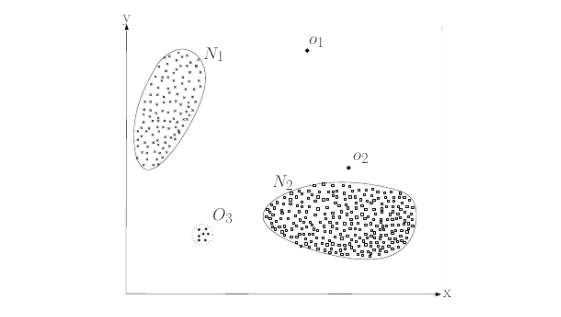
\includegraphics[width=1\textwidth]{obrazky-figures/anomalie_2d_sade.png}
\caption{Ukážka anomálií v 2D dátovej sady\cite{Chandola}}
\centering
\label{2d}
\end{figure}
\subsection{Kontextové anomálie}
Ak je v dátovej sade anomália iba v nejakom špecifickom kontexte, ale nie inak, navývame túto anomáliu ako kontextovú anomáliu. Pojem kontextu je predstavený v štruktúre dátových setov a musí byť špecifikovaný ako časť problému. Každá dátová inštancia je definovaná týmito vlastnosťami:
\begin{itemize}
    \item Kontextuálne vlastnosti sa používajú, aby určili kontext pre inštanciu. Napríklad v časovo sledovaných dátach je čas kontextová vlastnosť, ktorá určuje anomálie v čase.
    \item Vlastnosti správania definujú nekontextové charakteristiky inštancie. Napríklad v dátovom sete opisujúce priemerné zrážky na celom svete, veľkosť zrážok na nejakom konkrétnom mieste je vlastnosť správania.
\end{itemize}
Jednotlivé anomálie sú detekované použitím vlastností správania v špecifickom kontexte. Dátová inštancia môže byť kontextuálna anomália v danom kontexte, ale identická dátová inštancia sa môže považovať ako normálna v rozdielnom kontexte. Táto vlastnosť je kľúčová pre identifikovanie kontextuálnych vlastností a vlastností správania pre detekovanie kontextuálnych anomálií.\par
Na obrázku \ref{kontext} môžeme vidieť kontextovú anomáliu. Vidíme, že teplota $t_1$ je taká istá ako teplota $t_2$, ale vyskytuje sa v rozdielnom kontexte a preto sa považuje iba $t_2$ ako anomália.\cite{Chandola}
 \begin{figure}[!ht]
 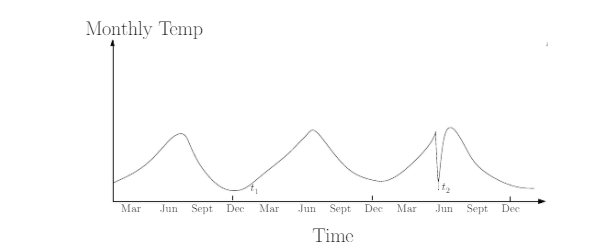
\includegraphics[width=1\textwidth]{obrazky-figures/kontext.png}
\caption{Kontextová anomália\cite{Chandola}}
\centering
\label{kontext}
\end{figure}

\subsection{Kolektívne anomálie}
Ak skupina dátových inštancií, ktoré majú podobné vlastnosti, sa chovajú anomálne k zvyšku dátovej sady, hovoríme, že ide o kolektívnu anomáliu. Ako ukážkový príklad si môžeme pozrieť sekvenciu akcií, ktoré sa vykonávajú v počítači:\par
. . . http-web, buffer-overflow, http-web, http-web, smtp-mail, ftp, http-web, ssh, smtp-mail, http-web, \textbf{ssh,buffer-overflow},ftp, http-web, ftp, smtp-mail,http-web . . .\par
Hrubom označená sekvencia udalostí ukazuje typický webový útok diaľkovým strojom, za ktorým nasleduje kopírovanie dát zo serveru do diaľkového stroja pomocou \emph{ftp}. Samotné udalosti anomáliu netvoria, iba keď sú za sebou alebo na rozličných miestach v sekvencii.\cite{Chandola}
\section{Označovanie dát anomáliou}  \label{Oznacovanie}
Dátová inštancia sa označuje ako normálna alebo anomálna. Často je zložité, aby sme presne dokázali označiť dáta ako normálne alebo anomálne. Preto je toto označenie robené zvyčajne ľudským expertom. Typicky je dané, že  označiť anomálne správanie v  sade anomálnych dátových inštancií, ktoré poskytujú všetky možné typy anomálneho správania, je zložitejšie ako označiť anomálne správanie pre normálne dátové inštancie. K tomu sa ešte  anomálne správanie môže meniť, vyvíjať a môžu sa vynájsť aj nové. Preto sa techniky detekcie anomálií delia do 3 módov:
\begin{enumerate}
    \item Detekovanie anomálií s dohľadom\par
    Techniky v móde s dohľadom predpokladajú, že tréningové dátové sady majú inštancie, ktoré sa rozdeľujú do normálnych alebo anomálnych tried. Typický prístup v týchto prípadoch je vybudovanie modelu normálnej triedy a anomálnej triedy. Každá dátová inštancia je porovnávaná týmto modelom, aby sa zistilo, do ktorej triedy patrí. Týmto prístupom sa vyskytujú dva hlavné problémy. Po prvé, anomálnych inštancií je počtom menej ako normálnych inštancií v tréningovej dátovej sade. Po druhé, je obtiažne  dosiahnuť presné a reprezentatívne označenie pre anomálnu triedu.
    \item Detekovanie anomálií s čiastočným dohľadom\par
    Techniky, ktoré pracujú v móde s čiastočným dohľadom predpokladajú, že tréningové dáta majú iba jednu normálnu triedu. Keďže nepotrebujú označenie pre anomálnu triedu, majú širšie využitie ako technika s plným dohľadom.
    \item Detekovanie anomálií bez dohľadu\par
    Techniky detekovania anomálií bez dohľadu nemajú žiadne tréningové dáta a preto sa využívajú najčastejšie. Tieto techniky implicitne predpokladajú, že normálne inštancie sa stávaju oveľa častejšie ako anomálie v testovacej sade. Ak je tento predpoklad nesprávny, potom táto technika má veľkú chybovosť.
    
\end{enumerate}\cite{Chandola}

\section{Techniky detekcie anomálií}
\subsection{Detekovanie anomálií založené na klasifikácií}
Metódy založené na klasifikácií fungujú v dvoj-fázovom režime. Trénovacia fáza učí klasifikátor (model) použitím dostupnou tréningovou sadou. Testovacia fáza potom klasifikuje testovaciu sadu ako normálnu alebo anomálnu použitím klasifikátora.\cite{Chandola} Techniky založené na klasifikácii sa spoliehajú na rozsiahle znalosti odborníkov o vlastnostiach sieťových útokov. Keď odborník na sieť poskytne detekčnému systému podrobnosti o charakteristikách útokov, je možné detekovať útok so známym vzorom hneď po jeho spustení. Výlučne to závisí od podpisu útoku ako od systému, ktorý je schopný detekovať útok, iba ak jeho podpis poskytol skôr sieťový expert. Toto demonštruje systém, ktorý dokáže zistiť iba to, o čom vie, že je škodlivé, a preto je  zraniteľný voči novým útokom, ktoré sa neustále objavujú v rôznych verziách a sú nenápadne spustené. Aj keď je podpis nového útoku vytvorený a zabudovaný do systému, počiatočná strata je nenahraditeľná a postup opravy je mimoriadne drahý.\cite{ahmed}\par

Metódy detekovania anomálií založené na klasifikácií fungujú na základe predpokladu, že klasifikátor, ktorý dokáže rozoznať medzi normálnou a anomálnou triedou, môže byť vytvorený na základe dostupných dát. Tieto techniky môžeme na základe tréningovej fázy rozdeliť  na dve kategórie:
\begin{itemize}
    \item Viac-triedne techniky na detekciu anomálií založené na klasifikácií predpokladajú, že tréningové dáta obsahujú prípady viacerých normálových tried. Tieto klasifikátory dokážu rozoznať medzi všetkými normálnými triedami. Ak ani jeden klasifikátor nedokáže zaradiť testovaciu inštanciu ako normálnu, táto inštancia je deklarovaná ako anomália.
    \item Jedno-triedne techniky na detekciu anomálií založené na klasifkácií predpokladajú, že všetky trénovacie inštancie majú iba jednu triedu. Tieto klasifikátory vytvárajú diskriminatívne hranice okolo normálnych inštancií. Hocijaká testovacia inštancia, ktorá nespáda do týchto hraníc, je považovaná za anomáliu.
\end{itemize}
\subsubsection{Neurónové siete}
Na detekciu anomálií, založených na klasifikácií, je možné využiť neurónové siete a to pri jedno-triednych,  ako aj pri viac-triednych nastaveniach. Viac-triedne techniky využívajú vo fáze tréningu neurónovú sieť na trénovanie na množine tréningových dát pre rozlíšenie rôznych tried. Potom je každá testovacia inštancia daná ako vstupné dáta do tejto neurónovej siete. Ak to neurónová sieť akceptuje, testovacia inštancia je normálová, ak nie, tak sme narazili na anomáliu. Jedno-triedne techniky používajú Replicator Neural Networks.\cite{Chandola}
\subsubsection{Bayesove siete}
Bayesova sieť je efektívny prístup k modelovaniu domény obsahujúcej neistotu. Diskrétna náhodná premenná je reprezentovaná pomocou smerovaného acyklického grafu (DAG), kde každý uzol odráža stav náhodnej premennej a obsahuje tabuľku podmienenej pravdepodobnosti (CPT). Úlohou CPT je poskytnúť pravdepodobnosť, že sa uzol bude nachádzať v konkrétnom stave. V Bayesovej sieti existuje medzi uzlami vzťah rodič-dieťa, čo naznačuje, že premenná predstavovaná podriadeným uzlom je závislá od tých, ktoré zastupujú nadradené uzly. Pretože táto sieť môže byť použitá pre schému klasifikácie udalostí, je použiteľná aj pre detekciu anomálií v sieti. V článku\cite{kruegel2003} sú identifikované dva hlavné problémy spôsobené vysoko falošnými pozitívami v technikách detekcie anomálií. Predpokladá sa, že systémy na zisťovanie anomálií obsahujú množstvo modelov na analýzu rôznych znakov udalostí. Prvým problémom je, že modely, ktoré poskytujú skóre alebo pravdepodobnosť normálnosti/abnormálnosti udalosti, vyžadujú, aby systém detekcie anomálií agregoval svoje rôzne výstupy, ktoré vedú k vysokým falošným pozitívam. Po druhé, systémy na zisťovanie anomálií nemôžu zvládnuť neobvyklé, ale legitímne správanie, napríklad náhle zvýšenie vyťaženia procesora, využitia pamäte atď. Ak sa vyskytne tento problém, ďalšie informácie vysvetľujú neobvyklé správanie, ktoré nie je neobvyklé.\cite{ahmed}

\subsubsection{Support Vector Machines}
Základný princíp Support Vector Machine (SVM) techniky je odvodiť hyperplán, ktorý maximalizuje separáčný okraj medzi normálnou a anomálnou triedou.\cite{eskin2002} Zaujímavá vlastnosť SVM techník je, že sa jedná o približnú implementáciu princípu minimalizácie rizika, založeného na teórii štatistického učenia. Štandardný algoritmus SVM je technika učenia pod dohľadom, ktorá na vytvorenie pravidla klasifikácie vyžaduje označené údaje. Môže sa však prispôsobiť ako algoritmus učenia bez dozoru, pričom sa pokúša oddeliť celú množinu tréningových údajov od ich pôvodu, zatiaľ čo bežný supervizovaný SVM sa pokúša oddeliť dve triedy dát v priestore funkcií pomocou hyperplánu.\cite{ahmed}\par

SVM techniky sa dajú aplikovať iba pri jedno-triednych  problémoch. Na sade označených trénovacích dát sa algoritmus natrénuje a vymedzí región, v ktorom sa
nachádzajú normálné dáta. Následne sa počas testovacej fázy algoritmus rozhodne, či skúmaná dátová inštancia do vymedzeného regiónu spadá alebo nie. Ak sa dátová inštancia nachádza
mimo vymedzeného regiónu, tak je označená za anomáliu.\cite{Chandola}
\subsubsection{Techniky založené na pravidlách}
Tieto techniky spočívajú vo vytvorení pravidiel, ktoré zachytávajú normálne správanie. Testované inštancie, ktoré nespĺňajú tieto pravidlá, sú označené ako anomálie. Táto technika je aplikovateľná ako pre jedno-triedne, tak aj pre viac-triedne nastavenia. Počas testovania je každej inštancii nájdené pravidlo, ktoré ju najlepšie popisuje a je jej priradené skóre rovné inverzií hodnoty istoty použitého pravidla. Jedno-triedne techniky používajú pravidlo Association rule mining pre tvorenie pravidiel bez dozoru.\cite{Chandola}\par
Klasifikačné techniky majú svoje dve veľké výhody, ale zároveň aj dve veľke nevýhody, na ktoré sa musí dať pozor pred tým, než ich použijeme. Medzi výhody patrí:
\begin{itemize}
    \item viac-triedne techniky dokážu využiť silné algoritmy na rozlišovanie medzi
jednotlivými triedami
    \item testovacia fáza je rýchla, nakoľko sa inštancia iba porovnáva s vytvoreným
modelom.
\end{itemize}
Medzi dve veľké nevýhody klasifikačných techník patrí:
\begin{itemize}
    \item  viac-triedne techniky sa spoliehajú na dostupnosť označených dát normálnych tried, čo je často nemožné
    \item výstupom väčšiny klasifikačných metód je označenie každej inštancie, čo vie
byť nevýhoda v prípadoch, kedy je vhodnejším výstupom skóre.

\end{itemize}
\cite{Chandola}
\subsection{Detekovanie anomálií založené na najbližšom susedovi}
Skupina metód založených na najbližšom susedovi pracuje s jedným základným
predpokladom, a to takým, že normálne dáta sa vyskytujú v hustých susedstvách, zatiaľ čo
anomálie sa vyskytujú osamote a ďaleko od akýchkoľvek iných dátových inštancií. Tieto techniky vyžadujú, aby bola vzdialenosť alebo podobnosť ako mierka na definovanie dvoch dátových inštancií. Túto vzdialenosť je možné vyrátať viacerými spôsobmi. Pre kontinuálne atribúty sa často používa Euklidovská vzdialenosť. Pre inštancie s viacerými atribútmi sú vzdialenosti zvyčajne počítané jednotlivo
pre atribúty a potom kombinovane.\cite{Chandola}\par
Medzi dva základné algoritmy patrí k-tý najbližši sused a relatívna hustota.
\subsubsection{K-tý najbližší sused}
Tento algoritmus je jeden z najznámejších a najviac používaných algoritmov pri detekcií anomálií
bez učiteľa. Sústreďuje sa na detekciu globálnych anomálií a nie je schopný detekovať
lokálne anomálie. Najprv sa pre každú dátovú inštanciu v datasete nájde k-najbližších
susedov a následne sa pre každý bod vypočíta hodnota (skóre), ktorá určí, či sa jedná
o anomáliu alebo nie.\cite{Chandola}
\subsubsection{Relatívna hustota}
Tieto techniky odhadujú
hustotu okolia všetkých inštancií. Inštancia, ktorá leží v riedkej oblasti, je
označená ako anomálna a inštancia z hustej oblasti normálna. Vzdialenosť
každej inštancie k jej k-tému najbližšiemu susedovi môže byť videná ako
inverzia hustoty okolia (k-tých inštancií) danej inštancie.
Tieto techniky nevykazujú dobré výsledky, ak dátová sada obsahuje
regióny s rôznymi hustotami inštancií. Tento problém je možné adresovať
technikami, ktoré počítajú hustotu okolia inštancie relatívne k hustotám okolitých inštancií.\cite{Chandola}\par
Problémom základnej techniky najbližšieho suseda je vysoká výpočtová náročnosť, ktorá sa dá do istej miery zmenšiť použitím komplexnejších štruktúr k-d stromov. Aj táto metóda prináša svoje výhody a nevýhody.\\
Výhody techník založených na najbližšom susedovi:
\begin{itemize}
    \item techniky bez dozoru nepotrebujú značené dáta a sú riadené čisto dátami
    \item techniky s čiastočným dozorom sú lepšie v ohľade neidentifikovaných anomálií, nakoľko pravdepodobnosť anomálie blízko testovacím dátam je nízka
    \item jednoduchá aplikácia na inú doménu - prevažne definovanie spôsobu merania
vzdialenosti.
\end{itemize}
Medzi nevýhody patrí:
\begin{itemize}
    \item pri technikách  bez dohľadu je možné, že normálne dáta nebudú
dostatočne blízko pri sebe a anomálie budú príliš blízko pri sebe, spôsobujúc
nesprávnu klasifikáciu
\item ak v technikách s čiastočným dozorom testované dáta nemajú dostatočnú
koncentráciu normálnych inštancii, je vysoký počet falošných pozitív
\item výpočtová náročnosť
\item definovanie spôsobu merania vzdialenosti môže byť náročné pre komplexné
dáta.
\end{itemize}


\subsection{Detekovanie anomálií založené na zhlukovaní}
Metódy detekcie anomálií v dátach založené na zhlukovaní sú používané takým
spôsobom, že najprv sa dáta rozdelia do zhlukov. Následne sa
pomocou vzdialenosti danej dátovej inštancie od centroidu rozhodne, či daný  bod je 
anomáliou alebo nie.\par
Na základe uvedeného predpokladu sa dajú tieto techniky rozdeliť do troch skupín:
\begin{enumerate}
    \item Normálne dátové inštancie patria do zhlukov, zatiaľ čo anomálie nepatria do žiadneho
zhluku. Tieto techniky používajú algoritmy, ktoré priradia inštancie do zhlukov, a tie, ktoré nepatria do žiadneho zhluku sú považované za anomálne. Nevýhodou týchto algoritmov je to, že nie vždy nájdu anomáliu, keďže tieto techniky sa zameriavajú na priradenie inštancií do zhlukov.
\item Normálne dátové inštancie ležia blízko ku \emph{stredu} ich najbližšieho zhluku a anomálie ležia ďaleko od \emph{stredu} ich najbližšieho zhluku. Techniky operujúce na tomto predpoklade
pozostávajú z dvoch krokov. V prvom kroku sú vytvorené zhluky zhlukovacím algoritmom. V druhom kroku je inštanciám pridelené skóre podľa ich
vzdialenosti od stredu ich najbližšieho zhluku.
\item Normálne dátové inštancie tvoria veľké a husté zhluky zatiaľ čo anomálie tvoria
malé alebo riedke zhluky. Techniky založené na tomto predpoklade označia
ako anomálie všetky inštancie, ktoré ležia v zhluku, ktorého veľkosť a/alebo
hustota je pod určenou hranicou alebo inak anomálna. 
\end{enumerate}

Výhody zhlukovacích metód sú nasledovné:
\begin{itemize}
    \item zhlukovacie metódy môžu fungovať samostatne
    \item sú adaptívne, dokážu pracovať jednoducho aj s komplexnými dátovými typmi
    \item časová zložitosť pre tréningovú fázu je rýchla, keďže počet zhlukov oproti jednotlivým inštanciam z testovacej sady je malý.
\end{itemize}
Nevýhody zhlukovacích metód:
\begin{itemize}
    \item efektivita a výkon týchto metód záleží na algoritme pre vytváranie zhlukov z normálových inštancií
\item mnohé techniky sú primárne zamerané na zhlukovanie a nie sú optimalizované na detekciu anomálií
\item viaceré metódy zhlukovania nútia, aby každá inštancia mala svoj zhluk; tým pádom sa môže vytvoriť veľký a široký zhluk, ktorý obsahuje aj anomáliu a potom nedokáže nájsť chybné inštancie
\item niektoré techniky sú efektívne, iba ak anomálie netvoria zhluky samé o sebe.
\end{itemize}
\cite{Chandola}
\subsection{Štatistické techniky detekcie anomálií}
Základný princíp, na ktorom fungujú každé štatistické techniky detekcie anomálií je, že kde normálne dáta sa vyskytujú vo vysoko pravdepodonostných regiónoch  stochaistického modelu a anomálie zase v nízkych pravdepodobnostných regiónoch tohto modelu. Štatistické techniky určia štatistický model (zvyčajne pre normálne správanie) a potom aplikujú štatistický interferenčný test, ktorý určí, či ďaľšie dátové inštancie patria do tohto modelu alebo nie. Dátové inštancie, ktoré majú nízku pravdepodobnosť vygenerovania sa do naučeného modelu, na základe aplikovaného štatistického testu, sú považované za anomálne. Existujú dve základné techniky, \emph{parametrické a neparametrické}.\cite{Chandola}

\subsubsection{Parametrické techniky}
Parametrické techniky predpokladajú, že normálne údaje sú generované parametrickým rozdelením s parametrami $\theta$ a funkciou hustoty pravdepodobnosti $f(x,\theta)$, kde 'x' je dátová inštancia. Skóre anomálie testovanej inštancie 'x'  je inverzná funkcia funkcie hustoty pravdepodobnosti, $f(x,\theta)$.  Parametre $\theta$ sú  odhadované z dostupných údajov. Alternatívne môže byť vykonaný štatistický test hypotéz. Nultá
hypotéza ($H_0$) pre takéto testy je, že inštancia dát x bola vygenerovaná pomocou
odhadovanej distribúcie (s parametrami $\theta$). Ak štatistický test zamietne $H_0$, 'x' je
vyhlásená za anomáliu. Test štatistickej hypotézy je spojený so štatistikou testu,
ktorú možno použiť na získanie pravdepodobnostného skóre anomálie pre inštanciu dát 'x'.
Na základe predpokladaného typu distribúcie môžu byť parametrické techniky ďalej
kategorizované :
\begin{itemize}
    \item Založené na Gaussovom modeli: Tieto techniky predpokladajú, že sú dáta generované z Gaussovej distribúcie.   Parametre tejto distribúcie vychádzajú z Maximum Likelihood Estimates (MLE). Vzdialenosť dátových inštancií od určeného priemeru je skóre anomálie pre dané dátové inštancie. Na stanovenie anomálií sa použije prahová (threshold) hodnota
anomálie. Rôzne techniky  vypočítajú vzdialenosť od priemeru a
prahovú hodnotu rôznymi spôsobmi.
\item Založené na regresnom modeli: Základná technika detekcie anomálií založená na regresnom modeli pozostáva z dvoch krokov.
V prvom kroku sa na dáta použije regresný model. V druhom kroku sa pre každý test, na stanovenie skóre anomálie, použije \emph{residual} (zostatok) pre testovaný prípad. Zostatok je taká časť dátovej inštancie, ktorá nie je popísaná v regresnom modeli.
\item Založené na zmesi parametrických techník distribucií: Takeéto techniky používajú na modelovanie údajov zmes parametrických štatistických distribúcií. Techniky v tejto kategórií môžu byť zoskupené do dvoch podkategórií. Prvá podkategória techník modeluje normálne dátové 
inštancie a anomálie ako samostatné parametrické distribúcie, zatiaľ čo druhá podkategória techník modeluje iba bežné inštancie ako zmes parametrických distribúcií.
\end{itemize} \cite{Chandola}
\subsubsection{Neparametrické techniky}
Techniky detekcie anomálií v tejto kategórii využívajú neparametrické štatistické modely, takže štruktúra modelu nie je aprioiri definovaná, ale je určená
z dátových inštancií. Takéto techniky zvyčajne vytvárajú menej predpokladov týkajúcich sa údajov,
napríklad hladkosť hustoty v porovnaní s parametrickými technikami.
\begin{itemize}
    \item Založený na histograme: Základná technika detekcie anomálií, založená na histograme pre jednorozmerné (majúce jednu vlastnosť) údaje, pozostáva z
dvoch krokov. Prvý krok spočíva v zostavení histogramu na základe rôznych hodnôt
z práve tejto vlastnosti v tréningových dátach. V druhom kroku technika skontroluje, či
testovacia inštancia spadá do ktorejkoľvek z košov (bin) histogramu. Ak áno, testovacia inštancia
je normálna, inak je anomálna. Variant základnej techniky založenej na histograme
je priradiť skóre anomálie každej inštancii testu na základe výšky (frekvencie)
koša, v ktorom sa nachádza.
Pre detekciu anomálií je kľúčová veľkosť koša použitého pri zostavovaní histogramu. Ak sú koše  malé, veľa normálnych testovacích prípadov bude spadať do prázdnych alebo unikátnych košov, čo bude mať za následok vo vysokej miere falošných poplachov. Ak sú koše veľké, veľa anomálnych testovacích inštancií
bude spadať do častých košoch, čo vedie k vysokej miere falošne negatívnych výsledkov. Preto je kľúčová výzva pre techniky založenými na histograme určenie optimálnej veľkosti košov, ktorý udržuje nízku mieru falošných poplachov a nízku mieru falošných negatívov.

\item Založené na funkciach kernela (jadra): Technika detekovania anomálií založená na funkciach kernela  zahŕňa použitie funkcií kernelu na aproximáciu skutočnej hustoty. Sú podobné parametrickým metódam opísaných vyššie. Jediným rozdielom je použitá technika odhadu hustoty.

\end{itemize} \par
Výpočtová zložitosť techník zisťovania štatistických anomálií závisí od povahy požadovaného štatistického modelu, ktorý zodpovedá dátovým inštanciam. Vybranie vhodných jednotlivých parametrických rozdelení z exponenciálnej triedy,
napríklad Gaussian, Poisson, Multinomial atď. sú zvyčajne lineárne z hľadiska veľkosti údajov, ako aj počtu atribútov. Prispôsobenie zložitých distribúcií (napríklad zmiešané modely,
HMM atď.) pomocou techník iteračného odhadu, ako je napríklad maximalizácia očakávaní
(EM), sú tiež zvyčajne lineárne pre jednotlivé iterácie, aj keď môžu konvergovať pomaly v závislosti od problému a/alebo kritéria konvergencie. Techniky založené na kernely môžu mať potenciálne  kvadratickú časovú zložitosť z hľadiska veľkosti údajov. \\
Výhody štatistických techník sú nasledovné:
\begin{itemize}
    \item Ak sú predpoklady týkajúce sa distribúcie základných údajov pravdivé, štatistické
techniky poskytujú štatisticky zdôvodniteľné riešenie na zisťovanie anomálií.
    \item Skóre anomálnej dátovej inštancie poskytnuté štatistickou technikou je spojené so spoľahlivosťou intervalu, ktorý je možné použiť ako ďalšiu informáciu pri rozhodovaní o ktorejkoľvek inštancii testu.
    \item Ak je krok odhadu distribúcie odolný voči anomáliám v dátach, štatistické techniky môžu pracovať v móde bez dohľadu.
\end{itemize}
Medzi nevýhody štatistických techník patria:
\begin{itemize}
    \item Kľúčovou nevýhodou štatistických metód je, že sa spoliehajú na predpoklad, že sú údaje  generované z konkrétnej distribúcie. Tento predpoklad často
neplatí, najmä pre viac-dimenzionálne dátove inštancie.
\item Zostrojenie hypotéznych testov na zložité distribúcie, ktoré sú potrebné na to, aby vyhovovali viac-dimenzonálnej dátovej sady, nie sú triviálne.
\item Techniky založené na histograme sa implementujú pomerne ľahko, ale kľúčovým nedostatkom týchto techník pre údaje s viac premennými je, že nie sú schopné zachytiť interakcie medzi rôznymi atribútmi. Anomálie môžu mať atribút
hodnoty, ktoré sú pre jednotlivé premenne veľmi časté, ale ktorých kombinácia je veľmi zriedkavá,  technika založená na histograme by však nebola schopná detekovať
takéto anomálie.
\end{itemize} \cite{Chandola}

\subsection{Informačno-teoretické techniky detekcie anomálií}
Informačno-teoretické techniky detekcie anomálií fungujú na predpoklade, že anomálne inštancie sa odlišujú od normálových v ich informačnom obsahu. Základná technika zahŕňa duálnu optimalizáciu, aby sa minimalizovala veľkosť podmnožiny a maximalizácia zníženia zložitosti dátových inštancií. Vyčerpávajúci prístup, pri ktorom sa zvažuje každá možná podmnožina dátových inštancií, má exponenciálnu časovú zložitosť. Tieto techniky sa tiež používaju v takých dátových množinách, kde sú jednotlivé dátové inštancie prirodzene usporiadané, napríklad sekvenčné alebo priestorové dáta. V týchto prípadoch sú jednotlivé inštancie rozdelené do sub-štruktúr a technika detekcie anomálií sa hľadajú v týchto sub-štruktúrach. \\
Výhody informačno-teoretických techník sú:
\begin{itemize}
    \item Môžu operovať v móde bez učiteľa.
    \item Nerobia predpoklady o štatistickej distribucií dátovej množiny.
\end{itemize} 

Nevýhody informačno-teoretických techník sú:
\begin{itemize}
    \item Výkon týchto techník veľmi závisí od voľby informačno-teoretickej mierky. Takéto opatrenia často dokážu zistiť prítomnosť anomálií, iba ak je v množine dát prítomný významne veľký počet anomálií.
    \item Techniky  aplikované na sekvencie alebo priestorové dáta sa spoliehajú na veľkosť sub-štruktúry, ktorá je často náročná na získanie.
\end{itemize} \cite{Chandola}

\subsection{Spektrálne techniky detekcie anomálií}
Spektrálne techniky detekcie anomálií sú založené na tom, že aproximujú dáta použitím kombinácií atribútov, ktoré zachytávajú rozsah rozličnosti dát. Tieto techniky ďalej pracujú s tým, že dáta môžu byť redukované na jednoduchšie dimenzie, kde sa ľahšie rozozná normálna dátová inštancia od anomálnej. Výhodami týchto metód je, že môžu fungovať v móde bez učiteľa, ale majú typicky veľkú výpočtovú náročnosť.\cite{Chandola}

\chapter{Umelá neurónová sieť}
\section{Čo je umelá neurónová sieť}
Umelá neurónová sieť je, ako indikuje jej meno, výpočtová sieť, ktorá sa pokúša simulovať proces rozhodnutí v sieťach nervovej bunky (neuróna) biologického centrálneho nervového systému. Táto simulácia je hrubá, bunka po bunke (neurón po neuróne, element po elemente) simulácia. Poznatky o koncepte tejto siete si vyberá z neurofyziologických poznatkov biologických neurónov a sietí, ako sú práve biologické neuróny. Tým sa líši od bežných  (digitálnych či analógových) výpočtových strojov, ktoré slúžia na nahradenie, vylepšenie alebo zrýchlenie výkonu ľudského mozgu bez ohľadu na organizáciu výpočtových prvkov a ich sietí. Musíme zdôrazniť, že táto simulácia neurónových sietí len veľmi hrubo kopíruje reálnu neurónovú sieť. Prečo vnímame  umelú neurónovú sieť viac ako len nejaké cvičenie v simulácií? Keďže to, čo dokáže spraviť umelá neurónová sieť, dokáže spraviť aj obvyklý digitálny počítač; aspoň teda výpočtovo.\cite{graupe}\par
Odpoveď na túto otázku pochádza najmä z dvoch hlavných aspektov. Umelá neurónová sieť, vytvorená simuláciou biologickej neurónovej siete, je v skutočnosti nová a neznáma počítačová architektúra s novými, neznámymi algoritmizáčnými technikami v porovnaní s obvyklými počítačmi. Tieto siete dokážu použitím veľmi jednoduchých výpočtových operácií (sčítavanie, násobenie a základné logické operácie) vyriešiť komplexné, matematicky zle-definované problémy, nelineárne problémy alebo stochaistické problémy. Obvyklý algoritmus využíva množiny operácií, ktoré aplikuje na daný problém. Vďaka tomu budú umelé neurónové siete výpočtovo a algoritmicky veľmi jednoduché a bude mať samo-organizujúcu funkciu, aby dokázali používať a uchovať tieto vlastnosti pre väčší rozsah problémov.\cite{graupe}

\section{Biologický a umelý neurón}
Činnosť nervovej sústavy je podmienená stavbou a funkciou jednotlivých nervových buniek a ich vzájomných vzťahov. V centrálnej nervovej sústave (CNS) vytvárajú nervové bunky komplikovanú a vzájomne mnohopočetnú prepojenú priestorovú sieť, v ktorej sú ako z funkčného, tak aj z morfologického hľadiska, v úzkom spojení gliové elementy.  Pojem neurón zahŕňa telo nervovej bunky aj s ich výbežkami ako na obrázku \ref{schema_neuronu}.\cite{otomar} \par
 \begin{figure}[!ht]
 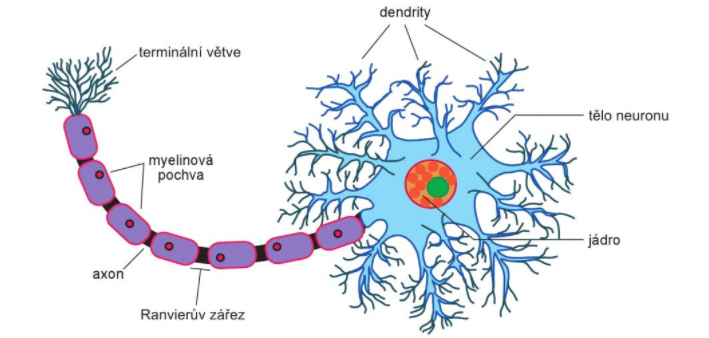
\includegraphics[width=1\textwidth]{obrazky-figures/schema_neuronu.png}
\caption{Schéma biologického neurónu\cite{otomar}}
\centering
\label{schema_neuronu}
\end{figure}
Neurón môžeme veľmi jednoduchým spôsobom, popísať ako jednotku, ktorá prijíma signály výbežkami zvanými \emph{dendrity}, kde sú spracované v jadre neurónu a výstup ide cez výbežok \emph{axón}. Dendritov má neurón typicky viac, bývajú kratšie a bohato sa vetvia na rozdiel od axónu, ktorý vedie ďalej od tela neurónu. Tento axón sa pripája na dendrity ďaľších neurónov. Neurón sa aktivuje a pošle signál cez axón do ďaľších neurónov, pokiaľ jeho dendrity dosiahnu, kombináciou vstupných parametrov, aktivačný potenciál\cite{otomar}. V skutočnosti je tento proces oveľa komplikovanejší. 
 \begin{figure}[!ht]
 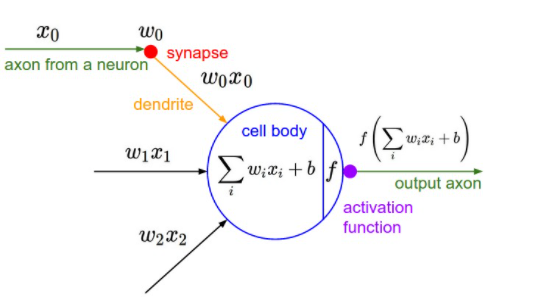
\includegraphics[width=1\textwidth]{obrazky-figures/neuron_mat.png}
\caption{Matematická schéma biologického neurónu\cite{stanford}}
\centering
\label{neuron_mat}
\end{figure}
Na obrázku \ref{neuron_mat} vidíme matematický, zjednodušený koncept biologického neurónu. Signál prechádza z axónu druhého neurónu ($x_0$), multiplikatívne interaguje ($w_0x_0$) s dendritami druhého neurónu na základe váhy synapsie (spojenia) ($w_0$). Koncept váhy týchto synapsií (označené $w$) sa dokážu učiť a kontrolujú silu influencie a jeho smeru (pozitívna váha alebo negatívna váha) jedného neurónu na druhý. Posledným parametrom tohto modelu je bias \emph{b}. Slúži na posun dát, aby sa lepšie hodila do  aktivačnej funkcie. V tomto základnom modeli, dendrity prenášajú signál do jadra neurónu, kde sú sčítané. Ak táto finálna suma je nad určeným thresholdom (prahová hranica), neurón sa aktivuje a vyšle signál po svojom axóne. Vo výpočtovom modeli predpokladáme, že nezáleží na presnom načasovaní aktivácie a že komunikáciu sprostredkuje iba frekvencia aktivácie. Na základe tejto frekvencii modelujeme aktiváciu neurónu s aktivačnou funkciou 'f', ktorá predstavuje frekvenciu aktivácií pozdĺž axónu. Z historického hľadiska je bežnou voľbou aktivačnej funkcie sigmoidná funkcia $\delta$, pretože vyžaduje vstup so skutočnou hodnotou (váha signálu po súčte) a stláča ho do rozmedzí od 0 do 1.\cite{stanford}

\section{Aktivačné funkcie umelého neurónu}
Umelé neuróny sa najviac rozlišujú aktivačnou funkciou. Ak sa táto aktivačná funkcia nepoužije v neurónovej sieti, výsledný signál je iba jednoduchá, lineárna funkcia, ktorá má polynomiálny stupeň jeden. Aj keď je lineárna rovnica  výpočtovo jednoduchá a riešiteľná, ich komplexita je limitovaná a nemajú možnosť sa učiť alebo rozoznať komplexné mapovanie z dát. Lineárne neurónové siete bez aktivačnej funkcie sa chovajú ako lineárne regresívne modely s limitovanou výkonnosťou. Tieto modely sú nedostatočné pre komplexnejšie výpočty, preto sa musia používať aktivačné funkcie . Medzi tieto aktivačné funkcie patrí:
\begin{itemize}
    \item binárna kroková aktivačná funkcia
    \item lineárna aktivačná funkcia
    \item sigmoidná aktivačná funkcia
    \item $tan_h$ aktivačná funkcia
    \item ReLU aktivačná funkcia
    \item leaky ReLU aktivačná funkcia
    \item parametrizovaná ReLU  aktivačná funkcia
    \item exponenciálna ReLU aktivačná funkcia
    \item SoftMax aktivačná funkcia
\end{itemize}
\cite{sharma}

\subsection{Binárna kroková aktivačná funkcia}
Binárna kroková funkcia je základná a najprimitívnejšia aktivačná funkcia ktorá existuje, a podarí sa ju naimplementovať iba pomocou if-else príkazov v Pythone. Veľkou nevýhodou je, že binárna kroková funkcia využíva binárny klasifikátor, preto  sa nemôže použiť v prípade multi-triednych klasifikácií. Takisto je gradient tejto funkcie 0, čo môže spôsobovať problém v spätnom propagačnom kroku. Matematicky sa definuje binárna kroková funkcia nasledovne: 
$$f(x) =
\left\{
	\begin{array}{ll}
		1  & \mbox{if } x \geq 0 \\
		0 & \mbox{if } x < 0
	\end{array}
\right.$$
\cite{sharma}

\subsection{Lineárna aktivačná funkcia}

Lineárna aktivačná funkcia je priamo úmerná k vstupným dátam. Najväčšou nevýhodou binárnej krokovej aktivačnej funkcie je, že má nulový gradient, lebo $x$ nemá žiaden multiplikátor. Toto sa dá odstrániť práve použitím lineárne aktivačnej funkcie, ktorá je matematicky definovaná nasledovne:
$$F(x) = ax$$
Veľkosť premennej $a$ môže byť ľubovolná a záleží na užívateľovi. V skutočnosti nie je veľkou výhodou používanie lineárnej aktivačnej funkcie, lebo neurónová sieť sa nebude zlepšovať na základe eroru kvôli rovnakej hodnote gradientu pre každú iteráciu. Takisto nie je schopná zachytávať komplexné vzorce v dátach. Preto sa lineárne aktivačné funkcie využívajú tam, kde je ľahká interpretovateľnosť a pre jednoduchšie zadania.\cite{sharma}


\subsection{Sigmoidná aktivačná funkcia}
Sigmoidná aktivačná funkcia je široko využívateľná, keďže  je to  nelineárna funkcia. Sigmodiná funkcia transformuje vstupné hodnoty do oboru hodnôt 0 až 1. Prakticky sa veľké negatívne hodnoty zobrazia v 0 a veľké pozitívne hodnoty zase v 1\cite{stanford}. Sigmoidná funkcia sa matematicky definuje ako:
$$F(x) = 1/e^{-x}$$\cite{sharma}

Táto funkcia sa čoraz menej používa kvôli dvom hlavným chybám:
\begin{itemize}
    \item Funkcia saturuje v hodnotách 0 a 1, kde je gradient  skoro nulový.
    \item Sigmoidné funkcie nie sú symetrické okolo 0, čo znamená, že znaky  všetkých výstupných hodnôt neurónu sú rovnaké. Tento problém ale môže byť napraviteľný úpravami sigmoidnej funkcie.
\end{itemize}\cite{stanford}

\subsection{TANH aktivačná funkcia}
Táto funkcia je \emph{hyperbolická tangent funkcia}, ktorá je podobná sigmoidnej funkcii, ale je symetrická podľa počiatku. Výsledky rozdielnych hodnôt výstupu z predošlej vrstvy budú dané ako vstupné hodnoty do ďaľšej. Matematicky je definovaná ako:
$$f(x) = 2sigmoid(2x)-1$$
$tan_h$ funkcia je súvislá a diferenciovateľná, jej hodnoty sú v obore hodnôt od -1 až 1. V praxi je táto funkcia viac preferovaná oproti sigmoid funkcii, keďže  má gradienty, ktoré nie sú obmedzené v určitom smere a je symetrická podľa počiatku.\cite{sharma} Na obrázku \ref{tan} \footnote{Zdroj:\url{https://en.wikipedia.org/wiki/Activation_function}}môžeme vidieť graf tejto funkcie.

\begin{figure}[!ht]
    \caption{Graf hypoerbolickej tangent funkcie}
    \centering
     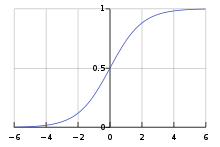
\includegraphics[width=0.5\textwidth]{obrazky-figures/tahn.png}
    \label{tan}
\end{figure}


\subsection{ReLU aktivačná funkcia}
ReLU - rectified linear unit, je nelineárna aktivačná funkcia, ktorá je široko využívaná v umelej neurónovej sieti. Výhodou použitia funkcie ReLU je, že všetky neuróny nie sú aktivované  súčasne. To znamená, že neurón bude deaktivovaný iba keď výstup lineárnej transformácie je 0. Matematicky sa zapisuje ako:
$$f(x) = max(0,x)$$
ReLU je efektívnejšia ako ďaľšie funkcie, pretože nie sú aktivované všetky neuróny naraz. Využíva sa pri spracovávaní obrazu, keďže ignoruje záporné hodnoty, čo je žiadúce pri práci s hodnotami pixlov.\cite{sharma} Na obrázku \ref{relu} \footnote{Zdroj:\url{https://medium.com/@danqing/a-practical-guide-to-relu-b83ca804f1f7}} vidíme graf tejto aktivačnej funkcie.
 \begin{figure}[!ht]
 \centering
 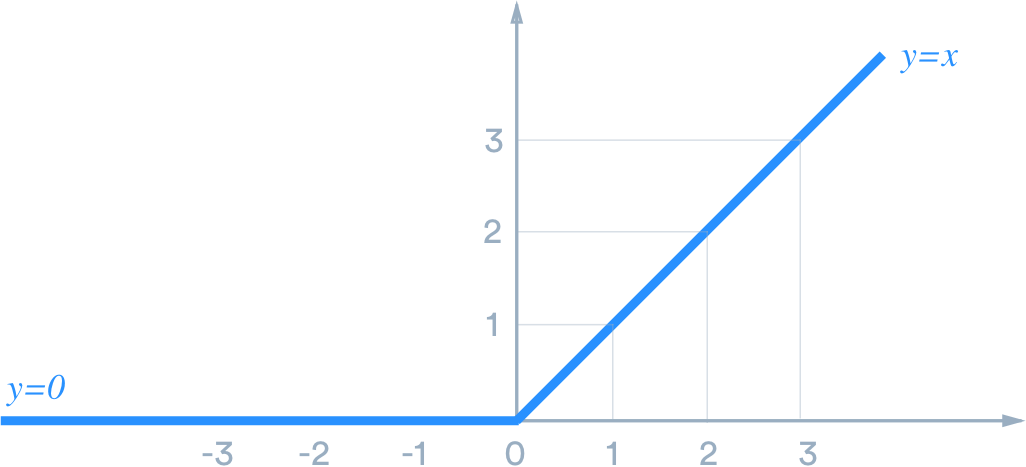
\includegraphics[width=0.5\textwidth]{obrazky-figures/relu.png}
\caption{Graf ReLU funkcie }

\label{relu}
\end{figure}
\subsection{Varianty ReLU aktivačných  funkcií}
Leaky ReLU je improvizaná ReLU funkcia, kde pre všetky negatívne hodnoty x je táto funkcia definovaná ako 'ax', kde a je extrémne malý parameter (0.01). Parametrizovaná ReLU sa líši od Leaky ReLU v parametri 'a', kde je nahradená ľubovoľným číslom.  Matematicky je definovaná ako:
$$f(x) =
\left\{
	\begin{array}{ll}
		x  & \mbox{if } x \geq 0 \\
		ax & \mbox{if } x < 0 ; a = 0.01 \text{ pre Leaky ReLU funkciu} 
	\end{array}
\right.$$ 
Pri parametrizovanej funkci sa tento parameter dokáže učiť.\par
Exponenciálna aktivačná funkcia využíva logaritmickú krivku pre definovanie záporných hodnôt; jej graf vidíme na obrázku \ref{erelu} \footnote{Zdroj: \url{https://machinelearningmastery.com/}}:
$$f(x) =
\left\{
	\begin{array}{ll}
		x  & \mbox{if } x \geq 0 \\
		a(e^x-1)x & \mbox{if } x < 0 
	\end{array}
\right.$$  \cite{sharma}
 \begin{figure}[!ht]
 \centering
 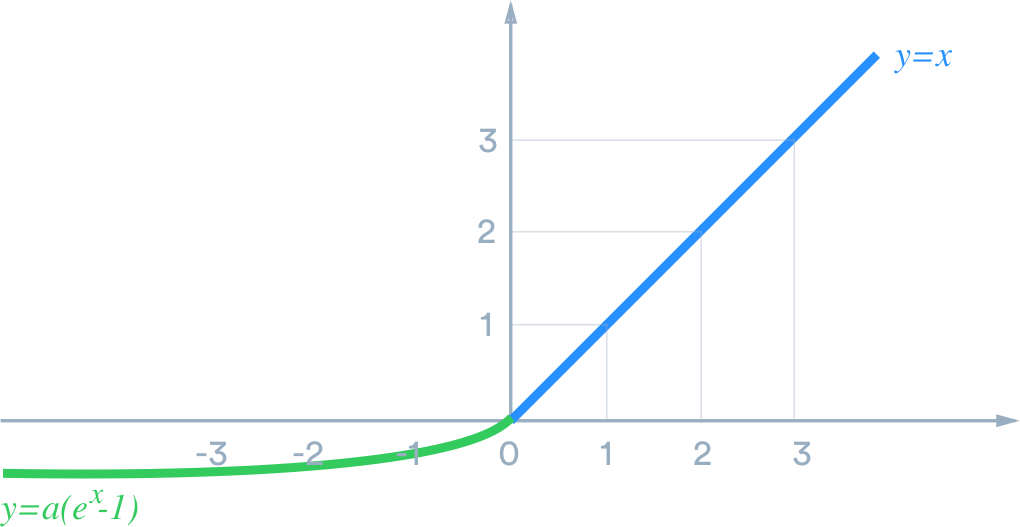
\includegraphics[width=0.5\textwidth]{obrazky-figures/e_relu.png}
\caption{Graf exponenciálnej ReLU funkcie }

\label{erelu}
\end{figure}
\subsection{SOFTMAX aktivačná funkcia}
SOFTMAX aktivačná funkcia je kombinácia viacerých sigmoidných funkcií. Sigmoidná funkcia, ako už bolo spomenuté, vracia hodnoty v intervale (0,1). Softmax funkcia na rozdiel od sigmoid funkcie sa môže použiť pre multi-triedne klasifikačné problémy. Využíva sa často v poslednej vrstve. Matematicky sa funkcia zapíše:
$$\delta(z)_j = \frac{e^{z_j}}{\sum_{k=1}^{K}e^{z_k}} for j=1,...K$$ \cite{sharma}

\section{Architektúra neurónovej siete}
Neurónové siete su modelované ako kolekcie umelých neurónov, ktoré su spojené do grafu. Dá sa povedať, že výstupy nejakých neurónov sa môžu stať vstupmi iných neurónov. Neurónové siete sú často rozdelené do distinktývnych vrstiev (layers). Pre bežnú neurónovú sieť, najbežnejšií typ vrstvy je \emph{plne-spojená vrstva}, v ktorej všetky neuróny z každej vrstvy sú spojené s neurónmi zo susednej vrstvy, ale tieto neuróny nie sú spojené v rámci jednej vrstvy. Na obrázku \ref{feed_n}\footnote{\url{https://ujjwalkarn.me/2016/08/09/quick-intro-neural-networks/}} vidíme necyklickú neurónovú sieť (feedforward neural network), tvoria ju 3 vstupné uzly, ktoré nie sú plne-spojené s druhou vrstvou, ktorá je skrytá. Výstupná vrstva má 2 uzly. Na obrázku \ref{cyclic_n}\footnote{\url{https://www.programmersought.com/article/6338898511/}} vidíme schému cyklickej neurónovej siete.\cite{karn}\par
Uzly v umelých neurónových sieťach sa delia na 3 typy:
\begin{itemize}
    \item Input (vstupné) uzly: tieto uzly v sebe nesú informáciu z vonkajšieho sveta do neurónovej siete a spoločne označené ako \emph{Input Layer (vstupná vrstva)}. Žiadne vypočítavanie sa v týchto uzloch nevykonáva, iba predajú informáciu ďalej do skrytých uzlov.
    \item Hidden (skryté) uzly: tieto uzly nemajú žiadne priame spojenie s vonkajším svetom, preto sa nazývajú skryté. Tieto uzly vykonávajú výpočet a transformujú informáciu zo vstupných uzlov do výstupných uzlov. Kolekcia týchto uzlov sa nazýva \emph{Hidden Layer (skrýta vrstva)}. Schémy môžu mať nula týchto vrstiev, jeden alebo aj viacej. 
    \item Output (výstupné) uzly: Tieto uzly majú na starosti vypočítanie a transformáciu z neurónovej sieti do vonkajšieho sveta. Kolekcia týchto uzlov sa nazýva \emph{Output Layer (výstupná vrstva)}.
\end{itemize}\cite{karn}\par



 \begin{figure}[!htb]
 \centering
 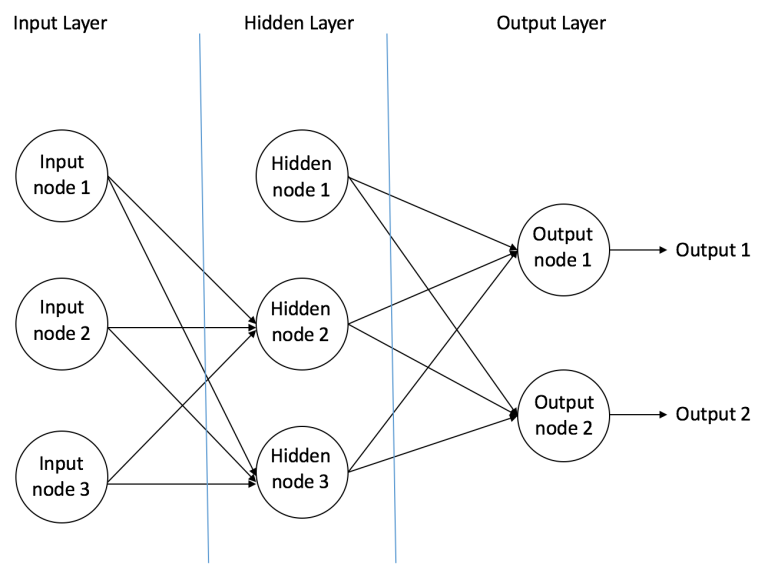
\includegraphics[width=0.5\linewidth]{obrazky-figures/feed_nw.png}
 \caption{Ukážka necyklickej neurónovej siete}

 \label{feed_n}
\end{figure}
 \begin{figure}[!htb]
 \centering
 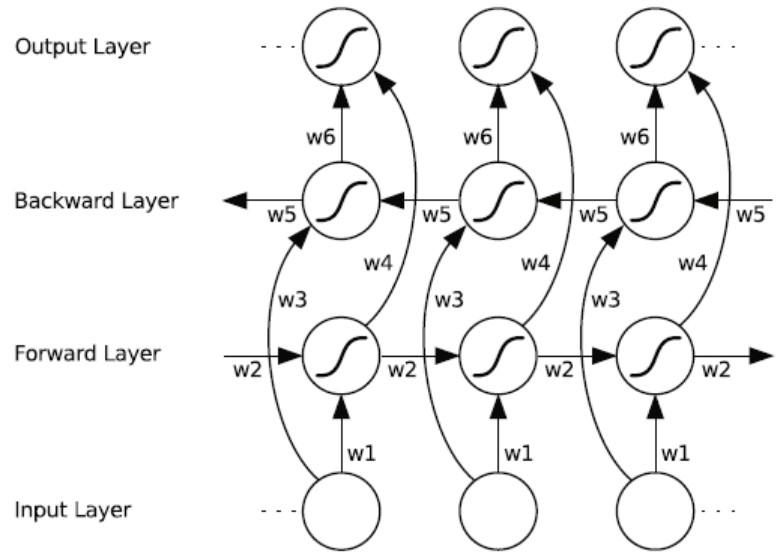
\includegraphics[width=0.5\linewidth]{obrazky-figures/cyclic_g.png}
 \caption{Ukážka cyklickej neurónovej siete}
 \label{cyclic_n}
\end{figure}

\section{Učenie sa umelej neurónovej siete}
Učenie sa umelej neurónovej siete sa dá pochopiť ako adaptácia tejto siete, aby lepšie zvládala problém na základe obhliadajúcich dát. V kapitole \ref{Oznacovanie} som poukázal na tri druhy učenia - s dohľadom, semi-dohľadom alebo bez dohľadu. Toto učenie upravuje váhy jednotlivých spojení medzi uzlami na zlepšenie výsledku. Zlepšnie sa robí najmä pomocou minimalizácie chybovosti. To však neznamená, že po úspešnom učení je táto chybovosť nulová. Ak je chybovosť veľmi vysoká, typicky sa musí zmeniť model neurónovej siete. 






\chapter{Návrh riešenia a implementácia}
\section{Vstupné dáta}
 Jeden z najdôležitejších aspektov pri detekovaní anomálií sú vstupné dáta. Ja som si ako vstupné dáta vybral dáta od kyberbezpečnostnej skupiny \emph{ Artificial Intelligence Centre}  na Českej Technickej univerzite v Prahe. Táto skupina je zameraná práve na kyberbezpečnosť, strojové učenie a pomáhanie druhým.\cite{strato} \par
 Technológia Stratosphere Intrusion Prevention System (Systém na prevenciu voči útokom) sa učí na modeloch vytvorených z reálnej zachytenej sieťovej prevádzky (ďalej len pcap), ktorá obsahuje škodlivé pakety. Práve používaním a študovaním týchto pcapov dokážu zaručiť, že jednotlivé vytvorené modely sú presné a ich úspešnosť je reálna. Ďaľši projekt vytvorený v tomto, tíme, \emph{Malware Capture Facility Project}, ktorý sa stará o konštatné monitorovanie hrozieb na internete a vytváranie škodlivých vzoriek, ktoré sa následne spustia na zariadeniach, ktoré zachýtavajú sieťovú prevádzku.\cite{strato}\par
 Algoritmy strojového učenia potrebujú dáta na učenie, testovanie a verifikovanie, aby zistili presnú výkonnosť na reálnych dátach. Mať dobré datasety je veľmi potrebné v sfére sieťovej bezpečnosti, keďze dáta v sieťach sú \emph{nekonečné}, meniace sa a rozličné. Preto na týchto stránkach nájdeme pcapy, ktoré zachytávajú normálnu prevádzku a pcapy, ktoré zachytávajú normálnu a malwarovú prevádzku.\cite{stratosphere}\par
 Jednotlivé pcapy, či už tie, ktoré zachytávajú normálnu alebo malwarovú prevádzku, potrebujem analyzovať a vytvoriť rozumný, použiteľný dataset. Pre zistenie malwarovej činnosti som sa rozhodol použiť technólogiu \emph{JA3 fingerprints}.
 \subsection{Ako funguje JA3}
 Transport Layer Security(TLS)\cite{TCP} je prenosový protokol, ktorý pracuje na vrchu TCP vrstvy, kde poskytuje bezpečnosť a integritu dát pre aplikácie, ktoré medzi sebou komunikujú. Protokol je rozdelený na dve časti:
 \begin{itemize}
  \item TLS Handshake Protocol
  \item TLS Record Protocol
\end{itemize}
TLS Handshake Protocol je zodpovedný za bezpečnostné parametre komunikácie; napríklad SSL verzia, metódy na výmenu kľúčov, zašifrovanie dát, autentizáciu, integritu dát, vlastnosti bezpečnostného kanálu.
TLS handshake komunikácia nie je zašifrovaná.\par
TLS Record Protocol zapúzdruje vysoko-úrovňové dáta a stará sa o posielanie zašifrované pakety. \cite{ja3}

 \begin{figure}[!ht]
 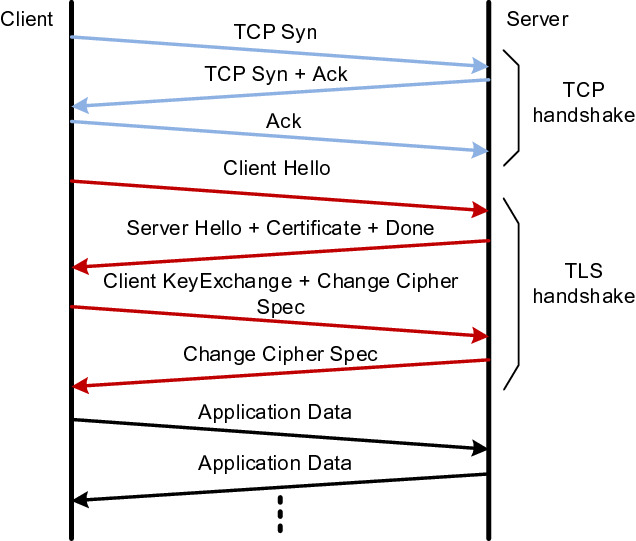
\includegraphics[width=1\textwidth]{obrazky-figures/tcp_tls.png}
\caption{Vytvorenie TLS spojenia\cite{ja3}}
\centering
\label{tcp_handshake}
\end{figure}
 Na obrázku \ref{tcp_handshake} vidíme, že pred TLS handshakom je najskôr TCP 3-way handshake. TCP vytvára také pripojenie, kde je potrebné vytvoriť spojenie ešte pred odosielaním dát. Najskôr si prijímajúca a odosielajúca strana zosychronizujú ich sekvenčné čísla, aby sa ich prenos mohol začať. Synchronizácia sa uskutočňuje výmenou segmentov, ktoré nesú synchronizačný bit (označovaný ako SYN). Synchronizácia vyžaduje, aby každá strana dostala potvrdenie tejto výmeny - acknowledgement (ACK). Celý tento mechanizmus sa realizuje v troch krokoch, preto sa nazýva 3-way handshake.\cite{trnav}\par
Po úspešnom vytvorení TCP pripojenia 3-way handshakom, TLS začne vytvárať bezpečnostné parametre použitím TLS Clienta (odosielateľa) a Server Hello paketov (prijímateľa). Klientská aplikácia ponúka sadu bezpečnostného zašifrovania a autetinzačné metódy použitím TLS Client Hello paketu. TLS server spracuje tieto vlastnosti komunikácie a pošle späť vlastnosti, ktoré sú podporované na serverovej strane. Server môže k tomu pripojiť serverový certifikát, aby mohol byť overený. Po ustanoveniach všetkých bezpečnostných parametrov, aplikačné dáta sa zapúzdrujú pomocou TLS Record Protocol a sú poslané po sieti.\cite{ja3}\par

Väčšina TLS fingerprint metód používa práve prvý paket poslaný klientom: Client Hello paket. Client Hello paket obsahuje TLS konfigurácie klientskej aplikácie, ktoré záležia od použitej TLS knižnice a operačného systému. Ako jeden príklad je výskum \emph{Network-Based HTTPS Client Identification Using SSL/TLS Fingerprinting}, kde okrem základných infromácií, akými je verzia TLS,  sa predovšetkým zamerali na zdieľanie starších protokolov.\cite{example} \emph{JA3} fingerprint je vyrobený  \emph{MD5} hashom z piatich TLS handshake polí:
\begin{itemize}
    \item TLS handshake version - TLS verzia aplikácie.
    \item Cipher suites - sada algoritmov, ktoré zvyčajne obsahujú algoritmy ako je výmena kľučov alebo message authentication code.
    \item Extensions - rozšírenia, ktoré boli prvý-krát predstavené v \emph{RFC 3456} a neskôr sa stali súčasťou TLS. Klient oznámi, ktoré rozšírenia podporuje a server potom vyberie, ktoré z týchto rozšírení sa použijú.\cite{extension}
    \item Supported Groupes(predtým Elliptic Curve) - algoritmy, ktoré šifrujú kľúče.\cite{ec}
    \item Elliptic Curve point format.

\end{itemize}
\cite{ja3}

\begin{figure}[!ht]
 \minipage{0.5\textwidth}
 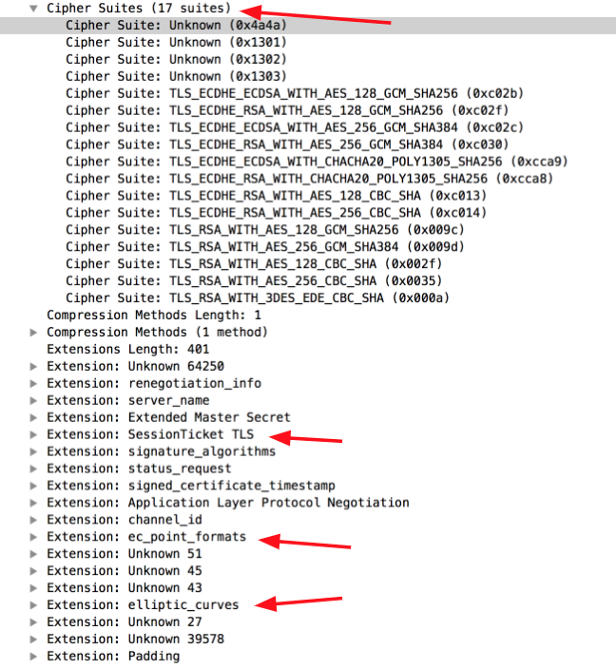
\includegraphics[width=\linewidth]{obrazky-figures/ja3_first.png}
 \endminipage
 \minipage{0.5\textwidth}
 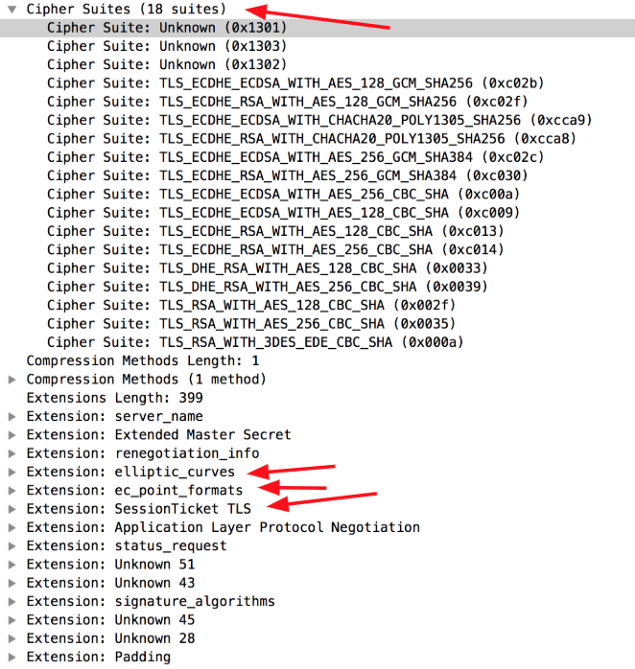
\includegraphics[width=\linewidth]{obrazky-figures/ja3_2nd.png}
 \endminipage
\caption{Vybrané polia zachytené v programe \emph{Wireshark}\cite{althouse}}
\centering
\label{ja3wireshark}
\end{figure}
\begin{figure}[!ht]
 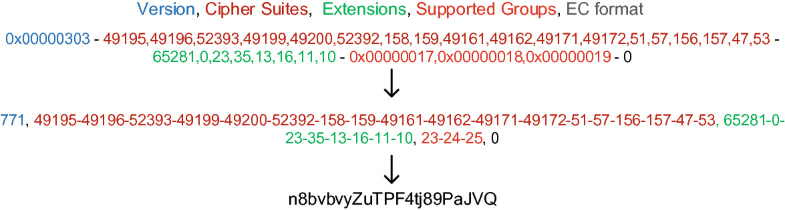
\includegraphics[width=1\textwidth]{obrazky-figures/ja3hash.png}
\caption{Vytvorenie JA3 hashu\cite{ja3}}
\centering
\label{ja3hash}
\end{figure}

Vytvorenie JA3 fingerprintu pozostáva z troch krokoch:
\begin{enumerate}
    \item Extrahovanie vybraných polí z TLS Hello paketu.
    \item Konkatenácia extrahovaných dát v decimálnych hodnotách; jednotlivé hodnoty polí sú oddelené pomlčkou a polia sú oddelené čiarkou.
    \item Aplikovanie MD5 hashovacieho algoritmu na vytvorený string.
\end{enumerate}

Výsledok je 32-bitový string v hexadecimálnej podobe. Na rozdiel od \emph{nmap} alebo fingerprint metódy webového prehliadača, JA3 fingerprint využíva viacej pasívny prístup. Proces vytvorenia TLS fingerprintov je rýchly, pretože pracuje iba s TLS hlavičkou. Bežne sieťové monitorovanie a IDS nástroje implementujú extrakciu TLS parametrov pre analýzu zašifrovanej sieťovej prevádzky. Aplikácia TLS fingerprintov na identifikovanie sieťových aplikácií vyžaduje, aby TLS fingerprint hodnoty boli jedinečné, presné a stále. Jeden z aspektov, ktoré limitujú spoľahlivosť TLS fingerprintov sú \emph{randomizované hodnoty v poli TLS Extensions}.\cite{ja3}
\subsubsection{Randomizované hodnoty v poli TLS Extensions}
V roku 2016 začal Google  generovať randomizované rozšírenia a zachovávať rozšíriteľnosť  (Generate Random Extensions And Sustain Extensibility - GREASE) hodnôt v TLS. GREASE hodnoty sú randomne generované čísla \emph{cipher suite, extensions} a \emph{supported groups}, ktoré sa nachádzajú v TLS Hello pakete. Slúžia na prevenciu chybovosti rozšíriteľnosti v TLS ekosystéme. Počas TLS handshake procesu, odpovedajúca strana musí ignorovať neznáme hodnoty. Účastníci, ktorý neignorujú tieto hodnoty, zlyhajú v inter-operácii, čo znamená bug v implementácii. Práve kvôli tomuto \emph{RFC 8701} pridala GREASE hodnoty ako časť zoznamu cipher suites, extensions a supported groups, na detekovanie neplatných implementácii.\cite{ja3}
\subsection{Vytorenie datasetu}
Dataset vytváram z pcap súborov. Zvolil som si, že škodlivé pakety budem určovať pomocou JA3 fingerprintov. Tieto fingerprinty sa nachádzajú len v TCP paketách, preto som si určil, že budem analyzovať \emph{TCP toky}.Vytvoril som si v pythone DataFrame, ktorý má nasledujúce polia:

\begin{itemize}
    \item index: určuje poradie TCP toku v pcape
    \item duration: celkové trvanie TCP spojenia v pcape
    \item srcIp: zdrojová IP adresa
    \item srdPort: zdrojový port
    \item dstIp: cieľová IP adresa
    \item dstPort: cieľový port
    \item service: protokol IP vrstvy
    \item srcBytes: počet bajtov poslaných zo zdrojovej IP adresy
    \item dstBytes: počet bajtov poslaných z cieľovej IP adresy
    \item flag: počet paketov, ktoré mali nastavený príznak \emph{TCP Reset}
    \item land: 1 ak je spojenie z rovnakého portu
    \item urgent: počet paketov, ktoré mali nastavený príznak \emph{TCP Urgent}
    \item ja3: Vytvorený JA3 fingerprint
    \item ja3Ver: SSL verzia v Client Hello pakete
    \item ja3Cipher: hodnoty jednotlivých ciphrov oddelené pomlčkou; keďže počet sa môže meniť, nastavil som, že ich je 35; tým pádom som buď doplnil nulami alebo odstránil hodnoty, ktoré pretiekli
    \item ja3Extension: hodnoty jednotlivých rozšírení oddelené pomlčkou; počet som nastavil na 25 a upravil; viď predchádzajúci riadok
    \item ja3Ec: hodnoty jednotlivých supported groups oddelené pomlčkou; počet som nastavil na 5 a upravil; viď predchádzajúci riadok
    \item ja3Ecpf:  hodnota eliptic curve point format; počet som nastavil na 2
    \item blacklisted: príznak, ktorý určuje, či je tok škodlivý
\end{itemize}
\cite{stolfo}\par
 Všetky polia, až na pole blacklisted,  zisťujem  analýzou pcap súborov pomocou pyshark knižnice. Nastavenie príznaku určujem na základe zisteného \emph{JA3
  fingerprintu}, ktorý porovnávam s databázou škodlivých JA3 fingerprintov. Pri zistení, že JA3 fingerprint sa nachádza v tejto databáze, označím priradený TCP tok ako škodlivý.
  
  
  \subsubsection{Vytvorenie blacklist databázy JA3 fingerprintov}
  Databázu \emph{blacklistdb} som vytvoril programom postgreSQL, kde som si vytvoril tabuľku \emph{ja3}. Dáta, t.j. JA3 fingerprinty, ktoré sú škodlivé. som použil z švajčiarskej stránky\footnote{\url{https://abuse.ch/}}, kde sa nachádza \emph{CSV} súbor škodlivých JA3 fingerprintov\footnote{\url{https://sslbl.abuse.ch/blacklist/ja3_fingerprints.csv}}. Tento súbor obsahuje nasledujúce polia:
  \begin{itemize}
      \item ja3\_md5: JA3 fingerprint
      \item Firstseen: kedy sa fingerprint prvý raz objavil na sieťach
      \item Lastseen: kedy sa fingerprint posledný raz objavil na sieťach
      \item Listingreason: dôvod, prečo je škodlivý 
  \end{itemize}
  Tabuľka má rovnakú štruktúru, akú má zmienený CSV súbor JA3 fingerprintov. Dáta som do nej naplnil pomocou skriptu napísaneho v jazyku \emph{Python}.
  
\section{Scikit-learn}

 
\section{Použité technólogie}
Pre celkovú implementáciu praktickej časti bakalárskej práce som sa rozhodol použiť programovací jazyk \emph{Python}. Python je vysoko-úrovňový programovací jazyk, ktorý je vhodný aj na písanie skriptov. Pre vytvorenie databázy som použil \emph{PostgreSQL}, kde mám vytvorenú tabuľku škodlivých JA3 fingerprintov. Na vkladanie dáta používam knižnicu \emph{psycopg2}. Pomocou tejto knižnice sa pripojím do už vytvorenej databáze a vložím potrebné údaje. Načítanie pcapov a analýzu paketov spracúvavam pomocou knižnice \emph{pyshark}, ktorý je obalom pre \emph{tshark}. Pyshark parsuje pakety použitím \emph{Wireshark dissectorov}. Analýzu jednotlivých TCP tokov skontrolujem práve pomocou programu \emph{Wireshark}. \par
Medzi ďaľšie použité knižnice používam \emph{os, hashlib, pandas, re...}

\chapter{Modelovanie a testovanie}
\chapter{Záver}

%===============================================================================
